% Provenance (never printed): see sources/outline_sources.md (Year 1:
% observational astronomy, photometry). Telescopes, angular resolution,
% gratings, the Doppler effect and the black-body laws are owned by the
% physics series and recalled here. Curves computed in
% figdata/bachelor-1/{blackbody_bands, extinction_line}.py; numbers of the
% exercises and problem in the Book 3 scratch calculator ch02.py.
\chapter{Télescopes, détecteurs et photométrie}\label{ch:b1:observing-the-sky}

Tout ce que l'astronomie sait des étoiles, à part quelques météorites et les
échantillons rapportés de la Lune et d'astéroïdes, elle l'a appris de la
lumière qu'elles envoient. Cette lumière traverse l'atmosphère terrestre, qui
absorbe des domaines entiers de longueurs d'onde et brouille le reste~; elle
est recueillie par un miroir dont la taille limite à la fois la faiblesse des
astres observables et la finesse des détails~; elle est comptée par un
détecteur qui transforme des photons en électrons, et chaque comptage porte une
incertitude statistique. Avant qu'un éclat devienne une \omterm{def:b1:observing-the-sky:flux}{luminosité} ou une
distance, chacune de ces étapes doit être comprise et corrigée. Ce chapitre
suit la lumière de l'étoile jusqu'au nombre~: les fenêtres de l'atmosphère et
la loi d'extinction, le télescope et le \omterm{def:b1:observing-the-sky:seeing}{seeing}, le détecteur et son bruit, puis
les magnitudes, les parallaxes et les couleurs qui transforment des \omterm{def:b1:observing-the-sky:flux}{flux}
mesurés en propriétés des étoiles. La même atmosphère, vue d'en bas, est
l'objet des chapitres sur le climat (\cref{ch:b1:radiation-heat-transport})~;
la même photométrie, appliquée aux planètes, ouvre le chapitre suivant
(\cref{ch:b1:comparative-planetology}).

\begin{recall}
L'objectif d'un télescope recueille la lumière sur son ouverture et forme une
image à son foyer~; la diffraction par une ouverture de diamètre $D$ limite le
plus petit angle qu'il sépare à environ $1.22\,\lambda/D$, critère de Rayleigh
(volume de physique de première année). Un réseau disperse la lumière selon la
longueur d'onde (deuxième année), et une source qui se déplace le long de la
ligne de visée voit ses raies spectrales décalées par l'effet Doppler
(année~12). Un corps en équilibre thermique émet le spectre du corps noir, dont
le maximum obéit à la loi de Wien (deuxième année). En chimie, l'absorbance
d'une solution croît proportionnellement à la longueur du trajet.
\end{recall}

\section{Les fenêtres de l'atmosphère}

L'atmosphère est transparente à certaines longueurs d'onde et opaque à
d'autres. Le rayonnement est absorbé surtout par la vapeur d'eau, le dioxyde de
carbone et l'ozone, et, aux plus courtes longueurs d'onde, par les atomes et les
molécules de la haute atmosphère elle-même.
% ledger: nasa:ems-absorbers

\begin{definition}[Fenêtre atmosphérique]\label{def:b1:observing-the-sky:window}
Une \emph{fenêtre atmosphérique}\index{fenetre atmospherique@fenêtre atmosphérique} est un domaine de longueurs d'onde dans lequel
l'atmosphère transmet la plus grande part du rayonnement qui arrive à son
sommet jusqu'au sol. La \emph{fenêtre optique} s'étend du proche ultraviolet au
proche infrarouge~; la \emph{fenêtre radio}, des longueurs d'onde d'environ un
centimètre à environ dix mètres.
\end{definition}

La figure ci-dessous esquisse l'opacité de l'atmosphère, des rayons gamma aux
grandes ondes radio. Les rayons gamma, les rayons X et l'ultraviolet en dessous
d'environ \qty{0.3}{\micro\metre} n'atteignent jamais le sol~: on les observe
depuis l'espace. La lumière visible passe, avec un certain flou. La plus grande
partie de l'infrarouge est absorbée par la vapeur d'eau et le dioxyde de
carbone, sauf dans des fenêtres étroites que les observatoires terrestres
exploitent sur des sites élevés et secs~; les \omterm{def:b1:observing-the-sky:magnitude}{bandes photométriques} du proche
infrarouge s'y logent, à \qty{1.24}{\micro\metre}, \qty{1.65}{\micro\metre} et
\qty{2.16}{\micro\metre}. Les longueurs d'onde d'environ
\qty{30}{\micro\metre} à un millimètre sont de nouveau bloquées~; les ondes
radio de quelques centimètres à une dizaine de mètres passent, même à travers
les nuages~; les plus longues sont réfléchies par l'ionosphère.
% ledger: nasa:opacity-windows, baldry:2mass-pivot

\begin{omfigure}
\begin{tikzpicture}[x=1.0cm, y=2.2cm, font=\scriptsize]
% x = log10(lambda / 1 m) + 10 ; opacity 0..1 (schematic, after the NASA figure)
\fill[omSea!20] (0,0) rectangle (13,1.05);
\fill[brown!50] (0,0) -- (0,1) -- (3.45,1) -- (3.52,0.05) -- (4.03,0.05)
  -- (4.06,0.6) -- (4.09,0.15) -- (4.15,0.6) -- (4.22,0.15) -- (4.28,0.6)
  -- (4.34,0.15) -- (4.42,0.7) -- (4.55,0.25) -- (4.65,0.8) -- (4.9,0.2)
  -- (5.12,0.2) -- (5.25,0.7) -- (5.4,1) -- (7.0,1) -- (7.3,0.6) -- (7.6,0.75)
  -- (8.0,0.5) -- (8.5,0.03) -- (11.0,0.03) -- (11.3,1) -- (13,1) -- (13,0)
  -- cycle;
\draw[black!70] (0,0) rectangle (13,1.05);
\foreach \x in {0,...,13} { \draw (\x,0) -- (\x,-0.05); }
\foreach \x/\l in {0/0.1 nm, 2/10 nm, 4/1 \unit{\micro m}, 6/100 \unit{\micro m}, 8/1 cm,
  10/1 m, 12/100 m}
  { \node[below] at (\x,-0.05) {\l}; }
\foreach \y/\l in {0/0, 0.5/50, 1/100}
  { \draw (0,\y) -- (-0.1,\y); \node[left] at (-0.1,\y) {\l}; }
\node[rotate=90] at (-0.75,0.5) {opacité (\%)};
\node at (6.5,-0.42) {\small longueur d'onde (échelle logarithmique)};
\node[align=center] at (1.7,0.75) {rayons gamma,\\ rayons X,\\ ultraviolet};
\node[align=center] at (6.2,0.75) {infrarouge\\ lointain};
\node[align=center] at (9.75,0.5) {fenêtre radio};
\node[omThm] at (4.15,0.86) {J H K};
\draw[-{Stealth}] (2.6,1.25) node[above] {fenêtre optique} -- (3.75,1.07);
\draw[-{Stealth}] (5.9,1.25) node[above] {fenêtres infrarouges} -- (4.6,1.07);
\end{tikzpicture}

{\small L'opacité de l'atmosphère au rayonnement venu de l'espace, de
\qty{0.1}{nm} à \qty{1}{km} (échelle logarithmique). Schéma d'après une figure
de la NASA tombée dans le domaine public~: seules comptent ici les fenêtres,
non la forme exacte de chaque bande d'absorption. J, H et K désignent les
\omterm{def:b1:observing-the-sky:magnitude}{bandes photométriques} du proche infrarouge.}
% ledger: nasa:opacity-windows, nasa:ems-absorbers, baldry:2mass-pivot
\end{omfigure}

\subsection*{Extinction}

Même à l'intérieur de la fenêtre optique, l'atmosphère retire une partie de la
lumière, par absorption et par diffusion sur les molécules et les aérosols. Une
couche mince d'épaisseur $\mathrm ds$ le long du rayon retire une fraction de
l'intensité proportionnelle à $\mathrm ds$~: $\mathrm dI = -\kappa I\,\mathrm ds$,
où le coefficient d'extinction $\kappa$ (par mètre) dépend de la longueur
d'onde et de la composition de l'air à cette altitude. C'est la loi de
l'absorbance d'une solution, appliquée à une colonne d'air.

\begin{proposition}[Loi de Bouguer]\label{prop:b1:observing-the-sky:bouguer}
Le long d'un rayon traversant un milieu absorbant, l'intensité décroît comme
\[
  I = I_0\,e^{-\tau}, \qquad \tau = \int_0^s \kappa\,\mathrm ds' ,
\]
où $I_0$ est l'intensité qui entre dans le milieu et $\tau$, l'épaisseur
optique du trajet, est un nombre pur.
Pour une atmosphère plan-parallèle, une étoile à la distance zénithale $z$
(angle entre sa direction et la verticale) est vue à travers l'épaisseur
optique $\tau(z) = \tau_0\sec z$, où $\tau_0$ est l'épaisseur optique au
\omterm{def:b1:spherical-astronomy:celestial-sphere}{zénith}.
\end{proposition}

\begin{proof}
L'équation $\mathrm dI/I = -\kappa\,\mathrm ds$ se sépare~: en intégrant du
sommet de l'atmosphère ($I = I_0$, $s = 0$) à l'observateur, on obtient
$\ln(I/I_0) = -\int_0^s\kappa\,\mathrm ds'$. Dans une atmosphère plan-parallèle,
$\kappa$ ne dépend que de la hauteur $y$, et un rayon incliné de $z$ sur la
verticale parcourt $\mathrm ds = \mathrm dy/\cos z$ pour s'élever de
$\mathrm dy$. D'où
$\tau(z) = \int \kappa(y)\,\mathrm dy/\cos z = \tau_0\sec z$.
\end{proof}

\begin{definition}[Masse d'air, coefficient d'extinction atmosphérique]\label{def:b1:observing-the-sky:extinction}
La \emph{masse d'air}\index{masse d'air} $X$ d'une observation est l'épaisseur
optique de la ligne de visée divisée par l'épaisseur optique au \omterm{def:b1:spherical-astronomy:celestial-sphere}{zénith}~:
$X = \tau(z)/\tau_0$. Elle vaut 1 au \omterm{def:b1:spherical-astronomy:celestial-sphere}{zénith} et, pour une atmosphère
plan-parallèle, $X = \sec z$. Le \emph{coefficient d'extinction
atmosphérique}\index{coefficient d'extinction atmospherique@coefficient d'extinction atmosphérique} $k$ dans une bande donnée est l'affaiblissement, en
magnitudes, produit par une masse d'air, de sorte qu'une étoile de magnitude
$m_0$ au-dessus de l'atmosphère est observée à
\[
  m = m_0 + kX .
\]
\end{definition}

Les magnitudes sont définies à la \cref{sec:b1:observing-the-sky:magnitudes}~;
il suffit ici de savoir qu'un affaiblissement d'un facteur $e^{-\tau}$ ajoute
$2.5\log_{10}e\;\tau = 1.086\,\tau$ magnitudes, de sorte que $k = 1.086\,\tau_0$.
La \omterm{def:b1:observing-the-sky:extinction}{masse d'air} plan-parallèle est excellente jusqu'à une hauteur d'environ
\ang{30} ($X = 2$) et tombe en défaut près de l'horizon, où $\sec z$ croît sans
limite alors que le trajet réel à travers une atmosphère courbe reste fini~;
les observateurs évitent les faibles hauteurs pour cette raison et pour le flou
qui croît avec le trajet.

\begin{method}[La droite d'extinction]\label{met:b1:observing-the-sky:extinction-line}
Pour trouver la magnitude $m_0$ qu'aurait une étoile au-dessus de l'atmosphère~:
\begin{enumerate}
  \item mesurer la magnitude $m$ de l'étoile, ou d'une étoile standard, à
        plusieurs \omterm{def:b1:observing-the-sky:extinction}{masses d'air} au cours de la nuit, pendant qu'elle se lève ou
        se couche~;
  \item calculer chaque \omterm{def:b1:observing-the-sky:extinction}{masse d'air} à partir de la distance zénithale,
        $X = \sec z$~;
  \item tracer $m$ en fonction de $X$ et ajuster une droite par moindres
        carrés~;
  \item la pente est le coefficient d'extinction $k$ de la nuit dans cette
        bande~; l'ordonnée à l'origine ($X = 0$) est $m_0$.
\end{enumerate}
Le même $k$ corrige ensuite toutes les autres étoiles observées la même nuit
dans la même bande~: $m_0 = m - kX$.
\end{method}

\begin{example}
Une nuit, une étoile a été mesurée six fois dans la bande V~:
\begin{center}
\small
\begin{tabular}{lcccccc}
\hline
$X$ & 1.05 & 1.18 & 1.36 & 1.62 & 1.95 & 2.31 \\
$m$ & 8.024 & 8.031 & 8.072 & 8.104 & 8.171 & 8.216 \\
\hline
\end{tabular}
\end{center}
La droite des moindres carrés, tracée dans la figure ci-dessous, a pour
pente $k = \qty{0.160}{\mag}$ par \omterm{def:b1:observing-the-sky:extinction}{masse d'air} et pour ordonnée à l'origine
$m_0 = 7.851$. Les points s'écartent d'elle de \num{0.006} magnitude, la
précision d'une bonne nuit de photométrie. Au \omterm{def:b1:spherical-astronomy:celestial-sphere}{zénith}, l'étoile est affaiblie de
\num{0.16} magnitude, soit une perte de
$1 - 10^{-0.4\times0.160} = \qty{14}{\percent}$ de sa lumière.
\end{example}

\begin{omfigure}
\begin{tikzpicture}
\begin{axis}[omrecord, width=0.62\linewidth, height=5.4cm, xmin=0, xmax=2.5,
  ymin=7.80, ymax=8.28, y dir=reverse, xlabel={masse d'air $X$},
  ylabel={magnitude $m$}, yticklabel style={/pgf/number format/fixed,
  /pgf/number format/precision=2}, tick label style={font=\scriptsize},
  label style={font=\small}]
\addplot[omThm, line width=0.9pt, dashed] table[x=X, y=m] {figdata/out/bachelor-1-extinction_line-fit.dat};
\addplot[only marks, mark=*, mark size=1.6pt, omDef] table[x=X, y=m] {figdata/out/bachelor-1-extinction_line-obs.dat};
\node[font=\scriptsize, right, fill=white, inner sep=1pt] at (axis cs:0.05,7.83) {$m_0 = 7.851$};
\node[font=\scriptsize, fill=white, inner sep=1pt, rotate=-10] at (axis cs:0.95,8.10) {pente $k = 0.160$};
\end{axis}
\end{tikzpicture}

{\small Une droite d'extinction~: la magnitude d'une étoile à six \omterm{def:b1:observing-the-sky:extinction}{masses d'air}
(points) et la droite des moindres carrés, extrapolée à $X = 0$, la magnitude
au-dessus de l'atmosphère. Les magnitudes croissent vers le bas~: une étoile
plus faible est plus bas.}
\end{omfigure}

\subsection*{Seeing}

L'air au-dessus d'un télescope n'est jamais immobile. Des cellules d'air de
températures légèrement différentes, donc d'indices de réfraction légèrement
différents, dérivent à travers le faisceau et le dévient de petits angles
aléatoires, qui changent plusieurs fois par seconde. L'œil voit une étoile
scintiller~; une longue pose enregistre une tache floue bien plus grande que la
figure de diffraction du télescope.

\begin{definition}[Le seeing]\label{def:b1:observing-the-sky:seeing}
Le \emph{seeing}\index{seeing} d'un site est le diamètre angulaire de l'image
d'une source ponctuelle brouillée par la turbulence atmosphérique en longue
pose, mesuré par la largeur à mi-hauteur de l'image, en secondes d'arc.
\end{definition}

Le \omterm{def:b1:observing-the-sky:seeing}{seeing} change d'une nuit à l'autre et d'une heure à l'autre. Les sites sont
choisis pour lui~: au sommet du Mauna Kea, à \qty{4204}{m}, le \omterm{def:b1:observing-the-sky:seeing}{seeing} médian de
l'atmosphère libre est d'environ \ang{;;0.40}, de \ang{;;0.45} environ en
hiver à \ang{;;0.35} en été, le meilleur dixième des nuits restant au-dessous
d'environ \ang{;;0.25}~; le même site n'a qu'une médiane de \qty{0.9}{mm} de
vapeur d'eau précipitable au-dessus de lui, ce qui ouvre ses fenêtres
infrarouges.
% ledger: cfht:site, cfht:seeing

\section{Télescopes et résolution}

Un télescope fait deux choses~: il collecte la lumière sur la surface de son
objectif, et il forme une image où les détails sont séparés. La surface
collectrice croît comme $D^2$~: un miroir deux fois plus large recueille
quatre fois plus de photons dans le même temps et atteint des étoiles quatre
fois plus faibles. La résolution est limitée par la diffraction à environ
$1.22\,\lambda/D$, et par le \omterm{def:b1:observing-the-sky:seeing}{seeing}.

\begin{example}
Le télescope Canada--France--Hawaï du Mauna Kea a une ouverture de
\qty{3.58}{m}. À \qty{550}{nm}, sa limite de diffraction est
\[
  1.22\times\frac{\qty{550e-9}{m}}{\qty{3.58}{m}} = \qty{1.87e-7}{rad}
  = \ang{;;0.039},
\]
dix fois plus fine que le \omterm{def:b1:observing-the-sky:seeing}{seeing} médian de \ang{;;0.40} du même site. Les
deux limites sont égales pour un miroir de diamètre $D = 1.22\lambda/\theta =
1.22\times\qty{550e-9}{m}/(\num{0.40}/\num{206265}) = \qty{0.35}{m}$~: tout
télescope au sol plus large qu'environ \qty{35}{cm} est limité par le \omterm{def:b1:observing-the-sky:seeing}{seeing},
et non par sa propre optique, aux longueurs d'onde visibles.
% ledger: cfht:aperture, cfht:seeing
\end{example}

Un grand télescope au sol gagne donc en surface collectrice, non en netteté, à
moins de corriger la turbulence. L'\emph{optique adaptative} le fait~: un
capteur mesure, plusieurs fois par seconde, la déformation du front d'onde d'une
étoile brillante (ou d'une étoile artificielle créée par un laser dans la haute
atmosphère), et un miroir mince, courbé par de nombreux petits actionneurs,
annule la déformation. La correction marche mieux dans
l'infrarouge, où la turbulence est plus lente et plus faible, et sur un petit
champ autour de l'étoile guide. Dans l'espace, il n'y a pas de \omterm{def:b1:observing-the-sky:seeing}{seeing} du tout.

\section{Détecteurs}

L'œil intègre la lumière pendant une fraction de seconde et ne répond qu'à une
petite fraction des photons qui y entrent. Les plaques photographiques
intégraient pendant des heures mais n'enregistraient qu'une petite fraction de
la lumière. L'astronomie moderne emploie des détecteurs de photons à
semi-conducteurs, où chaque photon absorbé d'énergie suffisante libère un
électron.

\begin{definition}[Rendement quantique, rapport signal sur bruit]\label{def:b1:observing-the-sky:detector}
Le \emph{rendement quantique}\index{rendement quantique} $\eta$ d'un détecteur à une longueur d'onde donnée est
la fraction des photons incidents qu'il enregistre, sous forme de
photoélectrons~: $\eta = N_\mathrm{e}/N_\gamma$. Le
\emph{rapport signal sur bruit}\index{rapport signal sur bruit} d'une mesure
est le signal mesuré divisé par son écart type, taille typique de son erreur
aléatoire.
\end{definition}

Le \emph{dispositif à transfert de charge} (CCD) est le détecteur standard de
la fenêtre optique. C'est une mince plaquette de silicium divisée en une grille
de pixels, chacun étant un puits de potentiel qui stocke les électrons libérés
par les photons absorbés en lui pendant la pose. À la fin de la pose, des
tensions appliquées en séquence aux électrodes déplacent les charges de pixel
en pixel, ligne par ligne, vers un amplificateur unique qui les mesure une à
une~; l'image est le tableau des comptages. Un CCD enregistre une grande
fraction des photons incidents sur la majeure partie du visible, sa réponse
est proportionnelle à la lumière reçue jusqu'à une charge maximale par pixel
(sa \emph{pleine capacité}), et il peut intégrer pendant des heures. Les
matrices infrarouges fonctionnent sur le même principe avec d'autres
semi-conducteurs, lues pixel par pixel.

Les photons arrivent au hasard. Si une source envoie en moyenne $N$
photoélectrons pendant une pose, le comptage effectivement enregistré fluctue
d'une pose à l'autre avec l'écart type $\sqrt N$ (statistique de Poisson,
admise en probabilités~: les comptages d'événements rares et indépendants).

\begin{proposition}[Bruit de photons]\label{prop:b1:observing-the-sky:snr}
Lorsque le bruit de photons de la source seule domine, une source donnant $R$
photoélectrons par seconde est mesurée en un temps $t$ avec le \omterm{def:b1:observing-the-sky:detector}{rapport
signal sur bruit}
\[
  \mathrm{SNR} = \frac{Rt}{\sqrt{Rt}} = \sqrt{Rt} ;
\]
il croît comme la racine carrée du temps de pose, et comme le diamètre du
télescope (puisque $R \propto D^2$). L'erreur sur la magnitude est alors
$\sigma_m \approx 1.086/\mathrm{SNR}$.
\end{proposition}

\begin{proof}
Le signal est $N = Rt$ et son écart type $\sqrt N$. Pour la magnitude,
$m = -2.5\log_{10}N + \text{cste}$, donc une petite erreur $\sigma_N$ donne
$\sigma_m = 2.5\log_{10}e\;\sigma_N/N = 1.086/\mathrm{SNR}$.
\end{proof}

Mesurer une magnitude à \num{0.01} près exige un \omterm{def:b1:observing-the-sky:detector}{rapport signal sur bruit}
d'environ 109, soit environ \num{12000} photoélectrons. Pour les sources
faibles, deux autres termes interviennent. Le ciel lui-même luit, et chaque
pixel de l'image de l'étoile collecte aussi des photons du ciel, à un taux $B$~;
et l'amplificateur ajoute un bruit de lecture $\sigma_r$ à chaque pixel lu.
L'expression complète,
\[
  \mathrm{SNR} = \frac{Rt}{\sqrt{Rt + Bt + n\sigma_r^2}}
\]
sur les $n$ pixels de l'image, se réduit à $\sqrt{Rt}$ pour une étoile brillante
et à $R\sqrt t/\sqrt B$ pour une source plus faible que le ciel. Comme $B$ croît
avec l'aire du disque de \omterm{def:b1:observing-the-sky:seeing}{seeing}, un bon \omterm{def:b1:observing-the-sky:seeing}{seeing} paie deux fois~: une image plus
nette sépare mieux et collecte moins de ciel (\cref{exo:b1:observing-the-sky:11}).

\begin{inthefield}[Une nuit au télescope]
La photométrie se fait avec des étalonnages autant qu'avec des étoiles. Avant
la nuit, un observateur d'un observatoire professionnel prend des images de
\emph{biais} (poses de durée nulle, qui enregistrent le décalage électronique
de chaque pixel) et des \emph{champs plats} (images de l'intérieur uniformément
éclairé de la coupole ou du ciel crépusculaire, qui cartographient la variation
de sensibilité d'un pixel à l'autre et à travers le champ)~; les images
scientifiques sont corrigées en soustrayant le biais et en divisant par le
champ plat. Pendant la nuit, des étoiles standard de magnitudes connues sont
observées à plusieurs \omterm{def:b1:observing-the-sky:extinction}{masses d'air} pour fixer la droite d'extinction et le point
zéro qui convertit les comptages en magnitudes. Une nuit est dite
\emph{photométrique} lorsque l'extinction reste assez stable pour que cette
correction tienne~; au sommet du Mauna Kea, \qty{55}{\percent} des nuits sont
photométriques.
% ledger: cfht:nights
\begin{center}
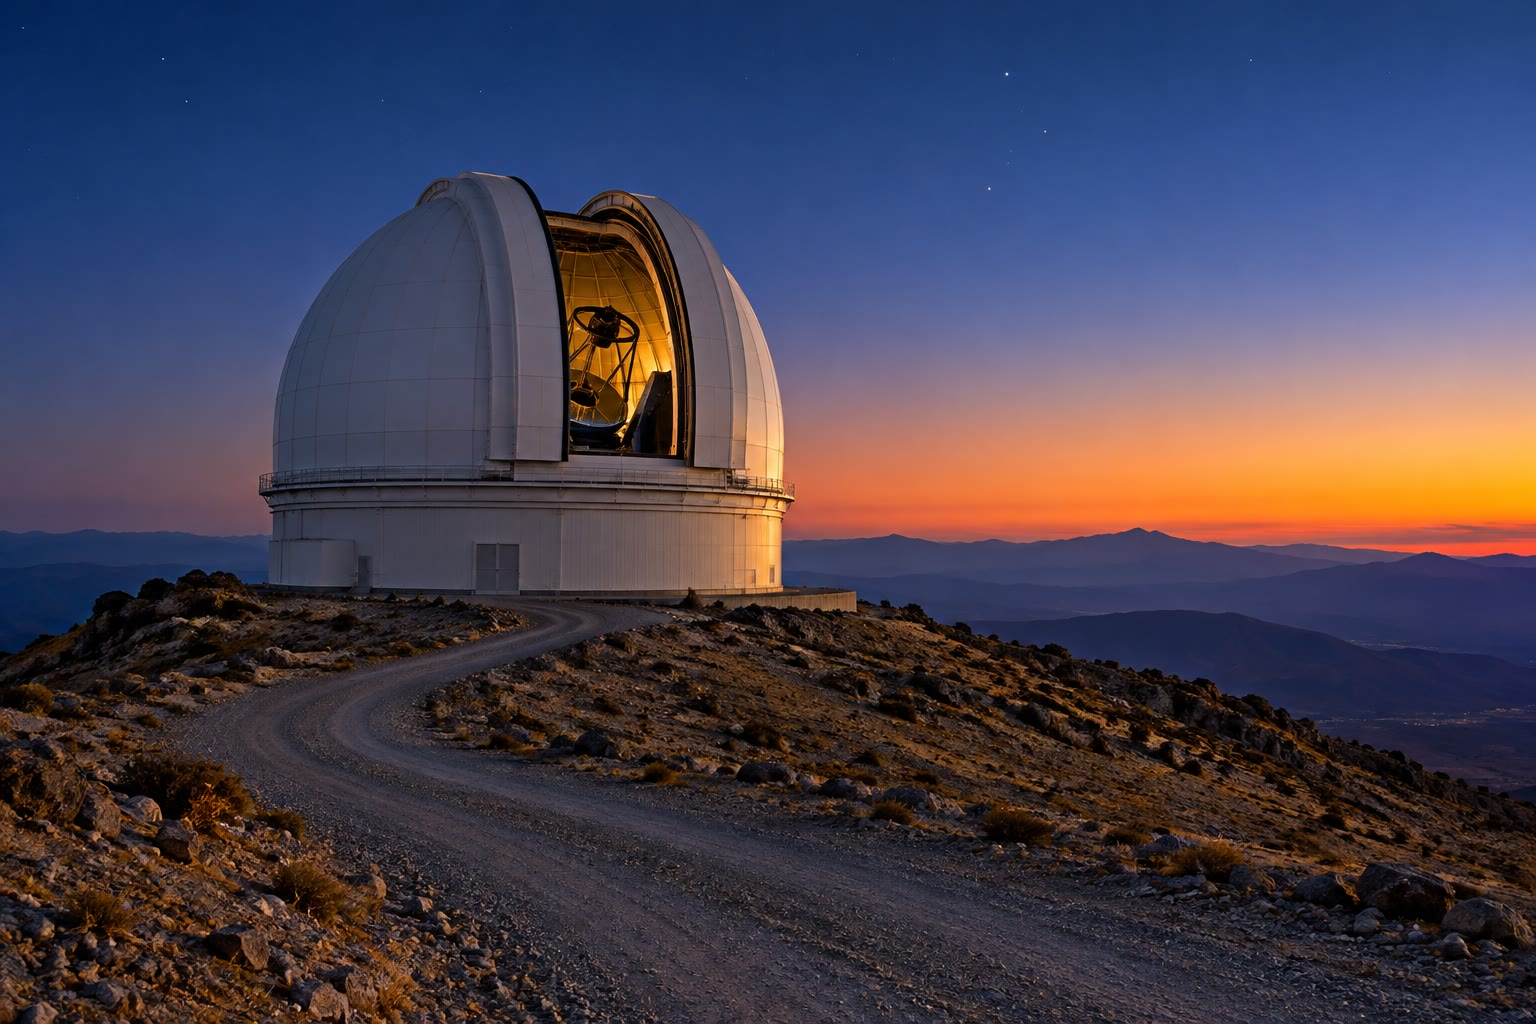
\includegraphics[width=0.55\linewidth]{images/book3/ai/b1-observatory-dusk.jpg}
\end{center}
\end{inthefield}

\section{Flux et magnitudes}\label{sec:b1:observing-the-sky:magnitudes}

\begin{definition}[Flux, luminosité]\label{def:b1:observing-the-sky:flux}
Le \emph{flux}\index{flux (d'une source)} $F$ reçu d'une source est la
puissance de son rayonnement traversant une surface unité perpendiculaire à sa
direction, en watts par mètre carré~; restreint à une bande de longueurs d'onde,
c'est le flux dans cette bande. La \emph{luminosité}\index{luminosite@luminosité} $L$ de
la source est la puissance totale qu'elle rayonne, en watts.
\end{definition}

\begin{proposition}[Loi en inverse du carré de la distance]\label{prop:b1:observing-the-sky:inverse-square}
Une source de \omterm{def:b1:observing-the-sky:flux}{luminosité} $L$ rayonnant également dans toutes les directions,
vue à une distance $d$ à travers le vide, donne le \omterm{def:b1:observing-the-sky:flux}{flux}
\[
  F = \frac{L}{4\pi d^2} .
\]
\end{proposition}

\begin{proof}
En régime stationnaire et sans absorption, la puissance qui traverse toute
sphère centrée sur la source est la même, $L$, par conservation de l'énergie.
Par symétrie, elle se répartit uniformément sur l'aire de la sphère, $4\pi d^2$.
\end{proof}

\begin{example}
La \omterm{def:b1:observing-the-sky:flux}{luminosité} du Soleil est de \qty{3.828e26}{W}. À une unité astronomique,
\qty{1.496e11}{m}, son \omterm{def:b1:observing-the-sky:flux}{flux} est $\num{3.828e26}/(4\pi\times
(\num{1.496e11})^2) = \qty{1361}{W.m^{-2}}$~: l'irradiance solaire que la
Terre reçoit au sommet de son atmosphère.
% ledger: sun:L, const:au, earth:TSI
\end{example}

Les \omterm{def:b1:observing-the-sky:flux}{flux} couvrent un énorme intervalle, et les astronomes les comparent sur une
échelle logarithmique héritée des classes dans lesquelles on rangeait jadis les
étoiles visibles à l'œil nu, les plus brillantes de première grandeur, les plus
faibles de sixième.

\begin{definition}[Magnitude apparente, bande photométrique]\label{def:b1:observing-the-sky:magnitude}
Une \emph{bande photométrique}\index{bande photometrique@bande photométrique} est un domaine de longueurs d'onde
sélectionné par un filtre standard, désigné par une lettre~: U (ultraviolet),
B (bleu), V (visuel), R (rouge), I (proche infrarouge), et J, H, K dans les
fenêtres de l'infrarouge. La \emph{magnitude apparente}\index{magnitude apparente} $m$ d'une source dans une
bande est définie à partir de son \omterm{def:b1:observing-the-sky:flux}{flux} $F$ dans cette bande par
\[
  m_1 - m_2 = -2.5\log_{10}\frac{F_1}{F_2} ,
\]
le point zéro étant fixé par des étoiles standard, proche de la magnitude de
l'étoile Véga dans chaque bande. Une différence de 5 magnitudes correspond à un
facteur exactement égal à 100 en \omterm{def:b1:observing-the-sky:flux}{flux}~; une magnitude est un facteur
$100^{1/5} = 2.512$. Les sources plus brillantes ont des magnitudes plus
petites, éventuellement négatives.
\end{definition}

Les longueurs d'onde pivots des filtres standard U, B, V, R et I sont
\qty{358.5}{nm}, \qty{437.1}{nm}, \qty{547.8}{nm}, \qty{650.4}{nm} et
\qty{802.0}{nm}.
% ledger: baldry:bessell-pivot
Dans la bande V, le Soleil a la \omterm{def:b1:observing-the-sky:magnitude}{magnitude apparente} $-26.74$, Sirius, l'étoile
la plus brillante du ciel nocturne, $-1.46$, et Véga $0.03$. Le Soleil est donc
$10^{0.4\times(26.74 - 1.46)} = \num{1.29e10}$ fois plus brillant que Sirius
dans notre ciel~; cela ne dit encore rien de celui des deux qui rayonne le plus,
ce qui exige les distances.
% ledger: nasa:sun-V, simbad:sirius, simbad:vega

\subsection*{Parallaxe et parsec}

Pendant que la Terre fait le tour du Soleil, une étoile proche semble se
déplacer par rapport aux étoiles de fond, bien plus lointaines, en décrivant en
un an une petite ellipse. Ce mouvement apparent est la mesure la plus directe
des distances stellaires~: il utilise l'orbite de la Terre comme base d'un
arpenteur.

\begin{definition}[Parallaxe annuelle, parsec]\label{def:b1:observing-the-sky:parallax}
La \emph{parallaxe annuelle}\index{parallaxe annuelle} $p$ d'une étoile est l'angle sous lequel on voit, depuis
l'étoile, le rayon de l'orbite de la Terre, soit une unité astronomique,
perpendiculairement à la ligne de visée~; c'est le demi-grand axe de l'ellipse
annuelle que l'étoile semble décrire. Le
\emph{parsec}\index{parsec} (\unit{\parsec}) est la distance à laquelle une
unité astronomique sous-tend une seconde d'arc~:
\[
  \qty{1}{\parsec} = \frac{\qty{1}{\au}}{\tan\ang{;;1}} = \qty{206265}{\au}
  = \qty{3.0857e16}{m} = \qty{3.2616}{\lightyear} .
\]
\end{definition}

Comme $p$ est minuscule, $\tan p \approx p$ en radians, et la distance s'ensuit
aussitôt~:
\[
  d = \frac{\qty{1}{\au}}{\tan p} \quad\Longrightarrow\quad
  \frac{d}{\unit{\parsec}} = \frac{1}{p/\text{arcsec}} .
\]
Sirius a une parallaxe de \ang{;;0.37921}, donc se trouve à $1/0.37921 =
\qty{2.637}{\parsec}$, soit \qty{8.60}{\lightyear}. Même les étoiles les plus
proches ont des parallaxes inférieures à une seconde d'arc, plus petites que le
\omterm{def:b1:observing-the-sky:seeing}{seeing}~: la parallaxe se déduit du déplacement du centre de l'image de l'étoile,
que de nombreux photons localisent bien plus précisément que la largeur de
l'image. Une mission spatiale décrite à la fin de ce chapitre a mesuré ainsi les
positions de près de deux milliards d'objets.
% ledger: simbad:sirius, const:au, esa:gaia

\begin{omfigure}
\begin{tikzpicture}[font=\small]
\draw[black!50] (0,0) ellipse (2.0cm and 0.55cm);
\fill[orange!80!black] (0,0) circle (3pt) node[below=3pt] {Soleil};
\fill[blue!70!black] (-2.0,0) circle (2pt) node[left, align=right] {Terre, six\\ mois plus tard};
\fill[blue!70!black] (2.0,0) circle (2pt) node[right] {Terre};
\fill (0,4.4) circle (1.6pt) node[above] {étoile};
\draw[omDef, thick] (0,0) -- node[right, pos=0.55] {$d$} (0,4.4);
\draw[omThm] (2.0,0) -- (0,4.4);
\draw[omThm, dashed] (-2.0,0) -- (0,4.4);
\draw[thick] (0,0) -- node[above] {\qty{1}{\au}} (2.0,0);
\draw[omThm] (0,3.75) arc[start angle=-90, end angle=-65.6, radius=0.65cm];
\node[omThm] at (0.17,3.38) {$p$};
\end{tikzpicture}

{\small \omterm{def:b1:observing-the-sky:parallax}{Parallaxe annuelle} (hors échelle)~: vue depuis l'étoile, le rayon de
l'orbite de la Terre sous-tend l'angle $p$. À six mois d'intervalle, la
direction de l'étoile diffère de $2p$. L'angle réel pour l'étoile la plus proche
est inférieur à une seconde d'arc.}
\end{omfigure}

\begin{definition}[Magnitude absolue, module de distance]\label{def:b1:observing-the-sky:absolute}
La \emph{magnitude absolue}\index{magnitude absolue} $M$ d'une étoile dans une
bande est la \omterm{def:b1:observing-the-sky:magnitude}{magnitude apparente} qu'elle aurait à la distance de
\qty{10}{\parsec}, vue à travers le vide. La différence $m - M$ est son
\emph{module de distance}\index{module de distance}.
\end{definition}

\begin{proposition}[Le module de distance]\label{prop:b1:observing-the-sky:modulus}
Pour une étoile à la distance $d$ vue à travers le vide,
\[
  m - M = 5\log_{10}\frac{d}{\qty{10}{\parsec}} .
\]
Si la lumière est affaiblie en chemin par $A$ magnitudes d'extinction,
$m - M = 5\log_{10}(d/\qty{10}{\parsec}) + A$. Dans une bande, le rapport des
\omterm{def:b1:observing-the-sky:flux}{luminosités} de deux étoiles est $L_1/L_2 = 10^{0.4(M_2 - M_1)}$.
\end{proposition}

\begin{proof}
D'après la loi en inverse du carré, le \omterm{def:b1:observing-the-sky:flux}{flux} à $d$ et le \omterm{def:b1:observing-the-sky:flux}{flux} à \qty{10}{\parsec}
sont dans le rapport $F(d)/F(\qty{10}{\parsec}) = (\qty{10}{\parsec}/d)^2$. La
définition des magnitudes donne $m - M = -2.5\log_{10}(\qty{10}{\parsec}/d)^2
= 5\log_{10}(d/\qty{10}{\parsec})$. L'extinction multiplie le \omterm{def:b1:observing-the-sky:flux}{flux} par
$10^{-0.4A}$, ce qui ajoute $A$ à $m$. À la distance commune de
\qty{10}{\parsec}, les \omterm{def:b1:observing-the-sky:flux}{flux} sont dans le rapport des \omterm{def:b1:observing-the-sky:flux}{luminosités}, et
$M_1 - M_2 = -2.5\log_{10}(L_1/L_2)$.
\end{proof}

Le Soleil a la \omterm{def:b1:observing-the-sky:absolute}{magnitude absolue} $M_\odot = 4.83$ et la \omterm{def:b1:observing-the-sky:flux}{luminosité}
\qty{3.828e26}{W}. En comparant la \omterm{def:b1:observing-the-sky:absolute}{magnitude absolue} d'une étoile dans V à celle
du Soleil, on obtient sa \omterm{def:b1:observing-the-sky:flux}{luminosité} dans V en unités solaires,
$L/L_\odot = 10^{0.4(4.83 - M)}$ --- une \omterm{def:b1:observing-the-sky:flux}{luminosité} \emph{en bande V}, car une
étoile bien plus chaude ou plus froide que le Soleil met une part différente de
sa puissance en dehors de la bande V.
% ledger: sun:Mabs, sun:L

\subsection*{Couleur}

\begin{definition}[Indice de couleur]\label{def:b1:observing-the-sky:colour-index}
L'\emph{indice de couleur}\index{indice de couleur} d'une étoile est la différence de
ses magnitudes dans deux bandes, la plus bleue en premier~; le plus utilisé est
$B - V$. Un $B - V$ petit ou négatif marque une étoile bleue, une valeur
grande une étoile rouge.
\end{definition}

L'\omterm{def:b1:observing-the-sky:colour-index}{indice de couleur} ne dépend pas de la distance, puisque la loi en inverse du
carré affaiblit les deux bandes de la même façon~; il mesure la forme du
spectre, donc la température de la surface de l'étoile. Une étoile rayonne à
peu près comme un corps noir dont le spectre culmine à
$\lambda_\mathrm{max} = b/T$ (loi de Wien, avec
$b = \qty{2.898e-3}{m.K}$, admise du volume de physique de deuxième année).
La figure ci-dessous trace trois spectres de corps noir~: un
corps froid à \qty{3500}{K} culmine dans le proche infrarouge et donne plus de
\omterm{def:b1:observing-the-sky:flux}{flux} dans V que dans B~; la température effective du Soleil, \qty{5772}{K}, place
son maximum à \qty{502}{nm}, entre B et V~; un corps à \qty{10000}{K} culmine
dans l'ultraviolet et est plus brillant dans B que dans V. Le rapport des
luminances B et V croît régulièrement avec la température, de \num{0.46} à
\num{0.97} puis \num{1.53} pour les trois courbes, ce qui explique que $B - V$
diminue quand $T$ augmente.
% ledger: const:b, nasa:sun-Teff, baldry:bessell-pivot

\begin{omfigure}
\begin{tikzpicture}
\begin{axis}[omrecord, width=0.9\linewidth, height=5.8cm, xmin=200, xmax=1500,
  ymin=0, ymax=1.17, xtick={200,400,...,1400}, ytick={0,0.5,1},
  xlabel={longueur d'onde (nm)},
  ylabel={$B_\lambda$ / maximum}, tick label style={font=\scriptsize},
  label style={font=\small}, legend style={font=\scriptsize, at={(0.5,1.03)},
  anchor=south, draw=none, fill=none}, legend columns=3]
\addplot[red!75!black, line width=1.1pt] table[x=lam_nm, y=t3500] {figdata/out/bachelor-1-blackbody_bands-curves.dat};
\addplot[orange!90!black, line width=1.1pt] table[x=lam_nm, y=t5772] {figdata/out/bachelor-1-blackbody_bands-curves.dat};
\addplot[omDef, line width=1.1pt] table[x=lam_nm, y=t10000] {figdata/out/bachelor-1-blackbody_bands-curves.dat};
\legend{\qty{3500}{K}, \qty{5772}{K} (le Soleil), \qty{10000}{K}}
\draw[black!45, densely dashed] (axis cs:358.5,0) -- (axis cs:358.5,1.06);
\node[font=\scriptsize, above, inner sep=1pt] at (axis cs:358.5,1.06) {U};
\draw[black!45, densely dashed] (axis cs:437.1,0) -- (axis cs:437.1,1.06);
\node[font=\scriptsize, above, inner sep=1pt] at (axis cs:437.1,1.06) {B};
\draw[black!45, densely dashed] (axis cs:547.8,0) -- (axis cs:547.8,1.06);
\node[font=\scriptsize, above, inner sep=1pt] at (axis cs:547.8,1.06) {V};
\draw[black!45, densely dashed] (axis cs:650.4,0) -- (axis cs:650.4,1.06);
\node[font=\scriptsize, above, inner sep=1pt] at (axis cs:650.4,1.06) {R};
\draw[black!45, densely dashed] (axis cs:802.0,0) -- (axis cs:802.0,1.06);
\node[font=\scriptsize, above, inner sep=1pt] at (axis cs:802.0,1.06) {I};
\end{axis}
\end{tikzpicture}

{\small Spectres de corps noir à trois températures, chacun divisé par son
propre maximum, avec les longueurs d'onde pivots des filtres U, B, V, R et I
(en tirets). Le maximum se déplace vers les courtes longueurs d'onde quand la
température augmente (loi de Wien)~: \qty{828}{nm}, \qty{502}{nm} et
\qty{290}{nm}.}
% ledger: const:h, const:c, const:kB, const:b, nasa:sun-Teff, baldry:bessell-pivot
\end{omfigure}

Quatre étoiles brillantes montrent l'éventail des couleurs~:
\begin{center}
\small
\begin{tabular}{lcccc}
\hline
étoile & $V$ & $B$ & $B - V$ & parallaxe (\unit{mas}) \\
\hline
Rigel & 0.13 & 0.10 & $-0.03$ & 3.78 \\
Altaïr & 0.76 & 0.98 & 0.22 & 194.95 \\
Polaris & 2.02 & 2.62 & 0.60 & 7.54 \\
Bételgeuse & 0.42 & 2.27 & 1.85 & 6.55 \\
\hline
\end{tabular}
\end{center}
% ledger: simbad:rigel, simbad:altair, simbad:polaris, simbad:betelgeuse
Rigel est blanc-bleu et Bételgeuse, dans la même constellation, orange-rouge~:
une différence de couleur visible à l'œil nu. Leurs types spectraux, B8 et
M1--M2, disent la même chose dans le langage des spectres, objet du volume de
troisième année.

\section{Spectrographes}

La photométrie mesure la lumière dans quelques larges bandes~; un spectrographe
l'étale en un spectre. La lumière issue du foyer du télescope traverse une fente
étroite, est rendue parallèle par un collimateur, est dispersée par un réseau
(ou un prisme) et est focalisée par une caméra sur un détecteur, où chaque
longueur d'onde tombe sur une colonne de pixels différente
(voir la figure ci-dessous). Un réseau dont $N$ traits
sont éclairés, utilisé à l'ordre $k$, sépare deux longueurs d'onde distantes de
$\Delta\lambda$ lorsque $\lambda/\Delta\lambda \le kN$, son pouvoir de
résolution (rappelé du volume de physique de deuxième année).

\begin{omfigure}
\begin{tikzpicture}[font=\scriptsize, >=Stealth]
\draw[thick, fill=omSea!25] (0.15,0) ellipse (0.13 and 0.9);
\node[below] at (0.15,-0.95) {objectif};
\draw[omDef] (-1.3,0.75) -- (0.15,0.75) -- (2.4,0);
\draw[omDef] (-1.3,-0.75) -- (0.15,-0.75) -- (2.4,0);
\draw[omDef, ->] (-1.3,0) -- (-0.2,0);
\node[above] at (-0.8,0.75) {lumière stellaire};
\draw[very thick] (2.4,-0.35) -- (2.4,-0.06); \draw[very thick] (2.4,0.06) -- (2.4,0.35);
\node[above] at (2.4,0.38) {fente};
\draw[omDef] (2.4,0) -- (3.6,0.55); \draw[omDef] (2.4,0) -- (3.6,-0.55);
\draw[thick, fill=omSea!25] (3.6,0) ellipse (0.1 and 0.72); \node[below] at (3.6,-0.74) {collimateur};
\draw[omDef] (3.6,0.55) -- (4.9,0.55); \draw[omDef] (3.6,-0.55) -- (4.9,-0.55);
\draw[thick, pattern=north east lines] (4.85,-0.8) rectangle (5.0,0.8);
\node[below] at (4.92,-0.82) {réseau};
\draw[blue!70!black] (5.0,0.3) -- (6.4,0.95); \draw[red!70!black] (5.0,0.3) -- (6.4,-0.15);
\draw[blue!70!black] (5.0,-0.3) -- (6.4,0.35); \draw[red!70!black] (5.0,-0.3) -- (6.4,-0.75);
\draw[thick, fill=omSea!25] (6.4,0.1) ellipse (0.1 and 1.08); \node[below] at (6.4,-1.0) {caméra};
\draw[blue!70!black] (6.4,0.95) -- (7.6,0.55); \draw[blue!70!black] (6.4,0.35) -- (7.6,0.55);
\draw[red!70!black] (6.4,-0.15) -- (7.6,-0.45); \draw[red!70!black] (6.4,-0.75) -- (7.6,-0.45);
\fill[black!70] (7.6,-0.8) rectangle (7.75,0.9);
\node[right, align=left] at (7.8,0.05) {détecteur~:\\ une longueur d'onde\\ par colonne};
\end{tikzpicture}

{\small Le trajet de la lumière dans un télescope et un spectrographe à réseau
(schématique, l'objectif du télescope et les optiques étant dessinés comme des
lentilles, avec deux longueurs d'onde)~: la fente isole l'image de l'étoile, le
collimateur rend le faisceau parallèle, le réseau le disperse, et la caméra
focalise chaque longueur d'onde en un point propre du détecteur.}
\end{omfigure}

Un spectre porte trois sortes d'information. Ses \emph{raies}, sombres là où
les atomes et les ions de l'atmosphère de l'étoile absorbent, brillantes là où
un gaz chaud et ténu émet, identifient les éléments chimiques présents. La
forme de son continuum, et les intensités relatives de raies formées à des
températures différentes, donnent la température du gaz. Et le décalage Doppler
des raies donne la vitesse le long de la ligne de visée~: une raie de longueur
d'onde au repos $\lambda$ est décalée de $\Delta\lambda = \lambda v_r/c$ pour
une vitesse radiale $v_r$ très inférieure à $c$. Mesurer $v_r$ à
\qty{1}{km.s^{-1}} exige un pouvoir de résolution de l'ordre de
$c/v_r = \num{300000}$, ou bien un pouvoir de résolution modéré et de nombreuses
raies mesurées ensemble. La façon dont les spectres révèlent la structure, la
composition et les mouvements des étoiles et des galaxies fait l'objet du
volume de troisième année.

\section{Observer depuis l'espace}

Au-dessus de l'atmosphère, il n'y a ni fenêtre fermée, ni extinction, ni
\omterm{def:b1:observing-the-sky:seeing}{seeing}, et, dans l'infrarouge, plus de lueur d'air tiède. Les télescopes
spatiaux paient cet avantage par leur coût, par la masse et la taille limitées
qu'une fusée peut lancer, et, pour la plupart, par l'impossibilité de les
réparer. On les emploie là où le sol ne peut rivaliser~: pour les rayons gamma,
les rayons X et l'ultraviolet, qui n'atteignent jamais le sol~; pour
l'infrarouge au-delà des fenêtres étroites~; pour des images à la limite de
diffraction sur un grand champ~; et pour des mesures, comme les parallaxes d'un
très grand nombre d'étoiles, qui exigent un instrument stable hors de l'air
turbulent.

\begin{dated}{2026}
% ledger: nasa:hubble-mirror, nasa:jwst-mirror, nasa:jwst-orbit, nasa:jwst-launch, nasa:jwst-range, esa:gaia
Trois observatoires spatiaux montrent l'éventail. Le télescope spatial Hubble,
lancé en 1990, a un miroir primaire de \qty{2.4}{m} de diamètre. Le télescope
spatial James Webb, lancé le 25 décembre 2021, a un miroir primaire de
\qty{6.5}{m} de diamètre formé de 18 segments hexagonaux, pour une surface
collectrice de \qty{25}{m^2}~; il travaille de \qty{0.6}{\micro\metre} à
\qty{28.5}{\micro\metre} et gravite autour du Soleil près du deuxième point de
Lagrange, L2, à \num{1.5} million de kilomètres de la Terre, du côté opposé au
Soleil. Gaia, lancé le 19 décembre 2013 vers la même région, a utilisé deux
télescopes sur un plan focal commun de CCD pour cartographier en trois
dimensions les positions et les mouvements de près de deux milliards d'objets~;
ses observations sont terminées, et ses catalogues sont en cours de
publication.
\end{dated}

\begin{omfigure}
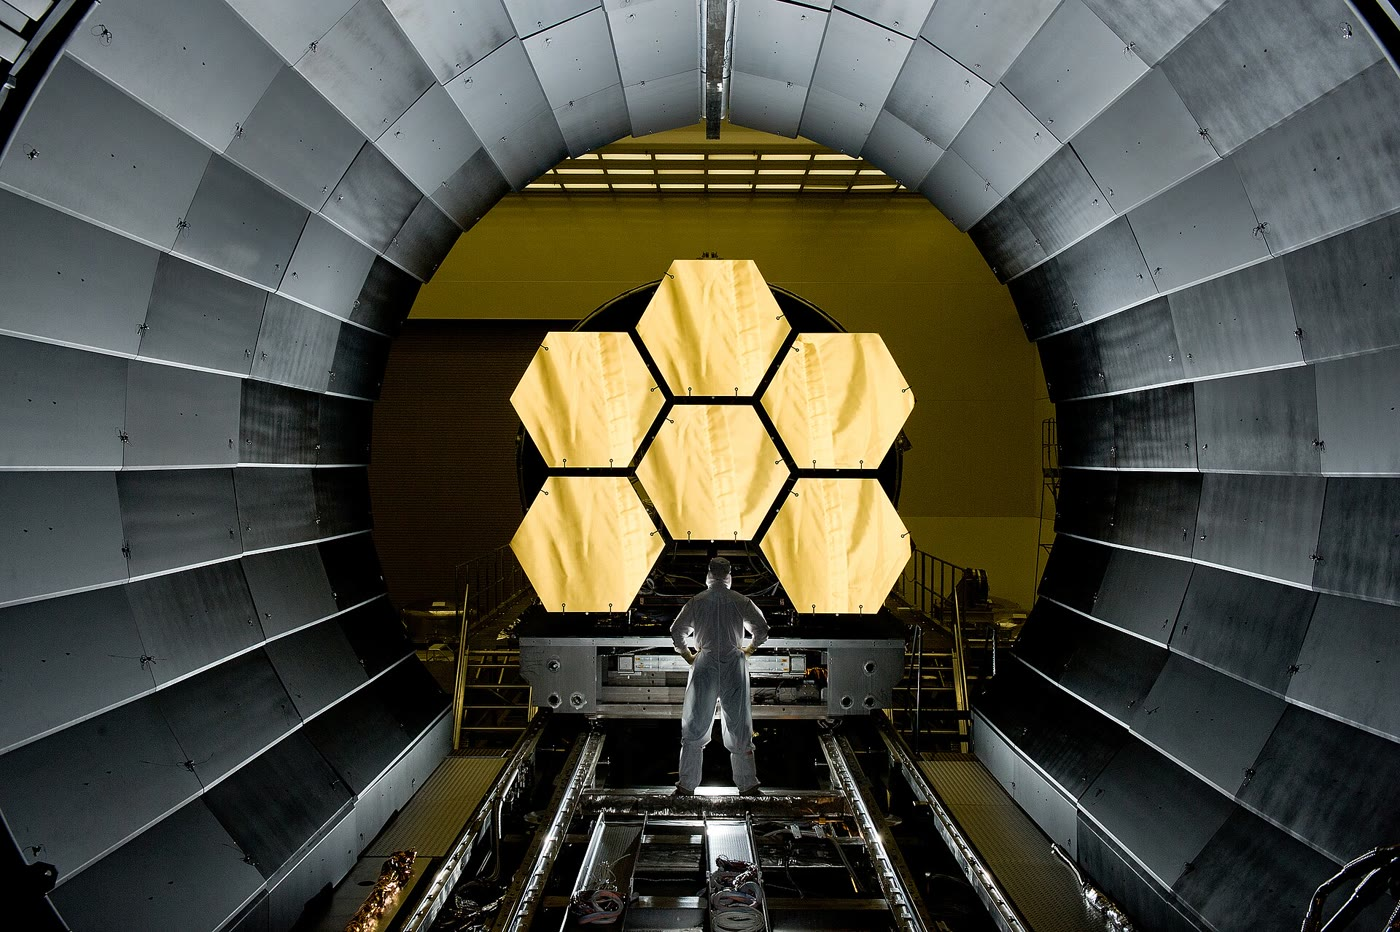
\includegraphics[width=0.78\linewidth]{images/book3/b1-jwst-mirror-segments.jpg}

{\small Six des 18 segments hexagonaux du miroir primaire du télescope spatial
James Webb, préparés pour un essai à froid en 2011~; ensemble, déployés dans
l'espace, les 18 forment un miroir de \qty{6.5}{m} de large. Photographie
NASA/MSFC/David Higginbotham, domaine public.}
% ledger: commons:jwst-mirror, nasa:jwst-mirror
\end{omfigure}

\section{Exercices}

\begin{exercise}[$\star$]\label{exo:b1:observing-the-sky:1}
Quel est le rapport des \omterm{def:b1:observing-the-sky:flux}{flux} de deux étoiles de magnitudes 1.0 et 6.0~? De
Rigel ($V = 0.13$) et de Polaris ($V = 2.02$)~? Laquelle est la plus brillante
dans le ciel~?
\end{exercise}

\begin{exercise}[$\star$]\label{exo:b1:observing-the-sky:2}
La parallaxe d'Altaïr est de \ang{;;0.19495}. Donner sa distance en \omterm{def:b1:observing-the-sky:parallax}{parsecs}, en
unités astronomiques et en années-lumière.
\end{exercise}

\begin{exercise}[$\star$]\label{exo:b1:observing-the-sky:3}
Calculer la limite de diffraction d'un télescope spatial de \qty{2.4}{m} à
\qty{550}{nm}, en secondes d'arc, et la comparer à un \omterm{def:b1:observing-the-sky:seeing}{seeing} de
\ang{;;0.40}. Faire de même pour un télescope de \qty{6.5}{m} à
\qty{2.0}{\micro\metre}.
\end{exercise}

\begin{exercise}[$\star$]\label{exo:b1:observing-the-sky:4}
À partir du tableau des quatre étoiles brillantes, classer Rigel, Altaïr,
Polaris et Bételgeuse de la surface la plus chaude à la plus froide. Pourquoi
peut-on comparer l'\omterm{def:b1:observing-the-sky:colour-index}{indice de couleur} entre des étoiles à des distances très
différentes~?
\end{exercise}

\begin{exercise}[$\star\star$]\label{exo:b1:observing-the-sky:5}
Une étoile est mesurée à la magnitude 6.412 à la distance zénithale \ang{30}
et à 6.590 à \ang{60} la même nuit. En supposant une atmosphère
plan-parallèle, calculer les deux \omterm{def:b1:observing-the-sky:extinction}{masses d'air}, le coefficient d'extinction et
la magnitude de l'étoile au-dessus de l'atmosphère.
\end{exercise}

\begin{exercise}[$\star\star$]\label{exo:b1:observing-the-sky:6}
Une étoile donne 400 photoélectrons en une pose de \qty{10}{s}, et le bruit de
photons de l'étoile seule domine. Quel est le \omterm{def:b1:observing-the-sky:detector}{rapport signal sur bruit}~?
Quelle durée de pose faut-il pour atteindre un \omterm{def:b1:observing-the-sky:detector}{rapport signal sur bruit} de
100~? Pour mesurer la magnitude à \num{0.01}~?
\end{exercise}

\begin{exercise}[$\star\star$]\label{exo:b1:observing-the-sky:7}
Rigel a $V = 0.13$ et une parallaxe de \ang{;;0.00378}. En négligeant
l'extinction entre Rigel et nous, calculer sa distance, sa \omterm{def:b1:observing-the-sky:absolute}{magnitude absolue} et
sa \omterm{def:b1:observing-the-sky:flux}{luminosité} en bande V en unités solaires ($M_\odot = 4.83$).
\end{exercise}

\begin{exercise}[$\star\star$]\label{exo:b1:observing-the-sky:8}
Comparer les surfaces collectrices d'un miroir circulaire de \qty{2.4}{m} (en
ignorant son obstruction centrale) et du télescope Webb (\qty{25}{m^2}). De
combien la pose pendant laquelle le télescope Webb recueille le même nombre de
photons est-elle plus courte~? Quelle fraction d'un disque plein de
\qty{6.5}{m} de diamètre sa surface collectrice représente-t-elle, et pourquoi
est-elle inférieure à un~?
\end{exercise}

\begin{exercise}[$\star\star$]\label{exo:b1:observing-the-sky:9}
(a) À partir de la \omterm{def:b1:observing-the-sky:flux}{luminosité} du Soleil, \qty{3.828e26}{W}, calculer son \omterm{def:b1:observing-the-sky:flux}{flux} à
\qty{10}{\parsec}. (b) Les \omterm{def:b1:observing-the-sky:magnitude}{magnitudes apparente} et absolue du Soleil sont
$-26.74$ et $4.83$. Utiliser le \omterm{def:b1:observing-the-sky:absolute}{module de distance} pour retrouver la distance
Soleil--Terre, en unités astronomiques.
\end{exercise}

\begin{exercise}[$\star\star\star$]\label{exo:b1:observing-the-sky:10}
Montrer à partir de la \cref{prop:b1:observing-the-sky:bouguer} que $k =
2.5\log_{10}e\;\tau_0$. Pour la nuit de la droite d'extinction ($k =
\num{0.160}$), calculer l'épaisseur optique au \omterm{def:b1:spherical-astronomy:celestial-sphere}{zénith} $\tau_0$ et la fraction de
la lumière qui atteint le télescope au \omterm{def:b1:spherical-astronomy:celestial-sphere}{zénith} et pour $X = 2.31$. Quelle \omterm{def:b1:observing-the-sky:extinction}{masse
d'air} prédirait une atmosphère plan-parallèle à une distance zénithale de
\ang{85}, et pourquoi ne faut-il pas se fier à cette valeur~?
\end{exercise}

\begin{exercise}[$\star\star\star$]\label{exo:b1:observing-the-sky:11}
Une galaxie faible donne $R = 50$ photoélectrons par seconde dans un télescope,
et le ciel dans l'aire de son image en donne $B = \num{2000}$ par seconde quand
le \omterm{def:b1:observing-the-sky:seeing}{seeing} est de \ang{;;0.80}. Le bruit de lecture est négligeable. (a) Combien
de temps faut-il poser pour un \omterm{def:b1:observing-the-sky:detector}{rapport signal sur bruit} de 10~? (b) Le ciel
dans l'image croît comme l'aire du disque de \omterm{def:b1:observing-the-sky:seeing}{seeing}. Recommencer pour un \omterm{def:b1:observing-the-sky:seeing}{seeing}
de \ang{;;0.40}. (c) Montrer que, pour une source très inférieure au ciel, le
temps de pose nécessaire pour un \omterm{def:b1:observing-the-sky:detector}{rapport signal sur bruit} donné varie comme
$\theta^2/D^2$, où $\theta$ est le \omterm{def:b1:observing-the-sky:seeing}{seeing} et $D$ le diamètre du télescope.
\end{exercise}

\begin{exercise}[$\star\star\star$]\label{exo:b1:observing-the-sky:12}
Un réseau de 1200 traits par millimètre est éclairé sur \qty{100}{mm} et
utilisé au premier ordre. (a) Quel est son pouvoir de résolution, et la plus
petite différence de longueur d'onde séparable à \qty{550}{nm}~? (b) À quelle
vitesse radiale cette différence correspond-elle~? (c) La Terre se déplace
autour du Soleil à \qty{29.78}{km.s^{-1}}. De combien ce mouvement peut-il
décaler une raie à \qty{550}{nm}, et à combien d'éléments de résolution cela
correspond-il~? Que doit donc faire un observateur qui mesure la vitesse d'une
étoile~?
% ledger: earth:vorb
\end{exercise}

\section{Problème~: Peser la lumière de Sirius}

\begin{problem}[{Problème du week-end --- la distance de Sirius, son éclat et le
nombre de photons qu'il envoie, et combien de soleils il éclipse}]
\label{pb:b1:observing-the-sky:1}
% ledger: simbad:sirius, simbad:vega, simbad:sirius-b, nasa:sun-V, sun:Mabs, const:au
% numbers computed in the scratch calculator calc/ch02.py from the rounded data
Sirius, l'étoile la plus brillante du ciel nocturne, a un compagnon faible, la
naine blanche Sirius~B. On utilise les données~:
\begin{center}
\small
\begin{tabular}{lcc}
\hline
astre & $V$ & parallaxe \\
\hline
Sirius & $-1.46$ & \ang{;;0.37921} \\
Sirius B & $8.44$ & --- \\
Véga & $0.03$ & \ang{;;0.13023} \\
le Soleil & $-26.74$ & --- \\
\hline
\end{tabular}
\end{center}
avec $M_\odot = 4.83$ dans V, $\qty{1}{\parsec} = \qty{206265}{\au} =
\qty{3.0857e16}{m} = \qty{3.2616}{\lightyear}$, et un coefficient d'extinction
$k = 0.15$ par \omterm{def:b1:observing-the-sky:extinction}{masse d'air} à l'observatoire.

\medskip
\noindent\textbf{Partie I --- À quelle distance est Sirius~?}
\begin{enumerate}
  \item Calculer la distance de Sirius en \omterm{def:b1:observing-the-sky:parallax}{parsecs}.
  \item L'exprimer en unités astronomiques et en mètres.
  \item L'exprimer en années-lumière. Il y a combien de temps la lumière que
        nous voyons ce soir a-t-elle quitté Sirius~?
  \item Sur une année, de quel angle total la direction de Sirius oscille-t-elle
        d'un côté à l'autre~? Le comparer à un \omterm{def:b1:observing-the-sky:seeing}{seeing} de \ang{;;0.40}.
        Pourquoi cette oscillation peut-elle pourtant être mesurée à une petite
        fraction du \omterm{def:b1:observing-the-sky:seeing}{seeing}~?
  \item Si la parallaxe était erronée de \ang{;;0.001}, de quelle fraction la
        distance serait-elle erronée, et de combien d'années-lumière~?
\end{enumerate}

\medskip
\noindent\textbf{Partie II --- Quel éclat a-t-il~?}
\begin{enumerate}[resume]
  \item Calculer le rapport des \omterm{def:b1:observing-the-sky:flux}{flux} de Sirius et de Véga dans V.
  \item Calculer le rapport des \omterm{def:b1:observing-the-sky:flux}{flux} du Soleil et de Sirius.
  \item Calculer le rapport des \omterm{def:b1:observing-the-sky:flux}{flux} de Sirius et de Sirius~B.
  \item Depuis l'observatoire du Paranal, Sirius traverse le méridien à une
        hauteur de \ang{82.09} (\cref{ch:b1:spherical-astronomy}). Calculer
        la \omterm{def:b1:observing-the-sky:extinction}{masse d'air}, l'extinction et la magnitude mesurée à cet instant.
  \item Recommencer à une hauteur de \ang{30}. Quelle fraction de la lumière
        est perdue en chemin~?
  \item Pourquoi la formule $X = \sec z$ tromperait-elle un observateur qui
        mesure Sirius juste après son lever~?
\end{enumerate}

\medskip
\noindent\textbf{Partie III --- Compter les photons.}
Une caméra montée sur un télescope de \qty{1}{m} enregistre $\num{3.0e4}$
photoélectrons par seconde d'une étoile de magnitude $V = 10.0$, une fois
corrigée de l'extinction. Chaque pixel contient au plus $\num{1.0e5}$ électrons
(sa pleine capacité).
\begin{enumerate}[resume]
  \item Combien de photoélectrons par seconde la caméra enregistre-t-elle de
        Sirius~B~?
  \item Quelle durée de pose donne à Sirius~B un \omterm{def:b1:observing-the-sky:detector}{rapport signal sur bruit} de
        1000, avec le seul bruit de photons de l'étoile~? Quelle est alors
        l'erreur sur sa magnitude~?
  \item Combien de photoélectrons par seconde la caméra enregistre-t-elle de
        Sirius~?
  \item Si \qty{20}{\percent} de la lumière de Sirius tombe dans son pixel le
        plus brillant, combien de temps ce pixel met-il à se remplir~?
  \item Sur l'image, les faibles ailes de l'image de Sirius déposent, à
        l'emplacement de Sirius~B, $10^{-4}$ de la lumière de Sirius par pixel,
        et le pixel le plus brillant de Sirius~B recueille \qty{20}{\percent} de
        sa propre lumière. Comparer les deux taux dans ce pixel.
  \item Quelle est la plus longue pose qui ne sature pas ce pixel~? Calculer le
        \omterm{def:b1:observing-the-sky:detector}{rapport signal sur bruit} de Sirius~B dans ce pixel pour une pose de
        \qty{0.5}{s}, en comptant le bruit de photons des deux sources. Sirius~B
        est-il détectable, et qu'est-ce qui rend la détection difficile~?
\end{enumerate}

\medskip
\noindent\textbf{Partie IV --- Combien de soleils~?}
\begin{enumerate}[resume]
  \item Calculer le \omterm{def:b1:observing-the-sky:absolute}{module de distance} de Sirius.
  \item En déduire la \omterm{def:b1:observing-the-sky:absolute}{magnitude absolue} de Sirius dans V, à deux décimales.
  \item Calculer la distance et la \omterm{def:b1:observing-the-sky:absolute}{magnitude absolue} de Véga.
  \item Lequel de Sirius et de Véga est intrinsèquement le plus lumineux dans V,
        et d'un facteur combien~?
  \item Quelle serait la \omterm{def:b1:observing-the-sky:magnitude}{magnitude apparente} du Soleil vu à la distance de
        Sirius~? En prenant 6.0 comme magnitude la plus faible visible à l'œil
        nu par nuit noire, serait-il visible~?
  \item Jusqu'à quelle distance Sirius resterait-il visible à l'œil nu~?
  \item Calculer la \omterm{def:b1:observing-the-sky:flux}{luminosité} de Sirius en bande V en unités solaires~:
        combien de soleils Sirius éclipse-t-il~?
\end{enumerate}
\end{problem}
